
\documentclass{article}
\usepackage{amsmath}
\usepackage{tikz}

\begin{document}

\begin{enumerate}
    \item A perfectly reflecting mirror of mass \( M \) mounted on a spring constitutes a spring-mass system of angular frequency \( \Omega \) such that \( \frac{4\pi M \Omega}{h} = 10^{24} \, m^{-2} \) with \( h \) as Planck's constant. \( N \) photons of wavelength \( \lambda = 8\pi \times 10^{-6} \, m \) strike the mirror simultaneously at normal incidence such that the mirror gets displaced by 1 \( \mu \)m. If the value of \( N \) is \( x \times 10^{12} \), then the value of \( x \) is \_\_\_\_. \\
    [Consider the spring as massless]
    \begin{center}
        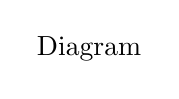
\begin{tikzpicture}
            \node {Diagram};
        \end{tikzpicture}
    \end{center}
\end{enumerate}

\end{document}
